% Exact finite example from Section 5: y=(0,2,4,6), M=4, n=2.
% Each list gives one estimate/vertical-offset pair per equally likely sample.
% Offsets separate duplicate estimates; only horizontal position encodes labour.
% Text alternative: the three estimators have common mean twelve but different
% spreads. Without predictions their estimates are 4,8,12,12,16,20. With the
% first prediction they are 8,12,12,12,12,16; with the second -4,4,12,12,20,28.
\begin{figure}[htp]
\centering
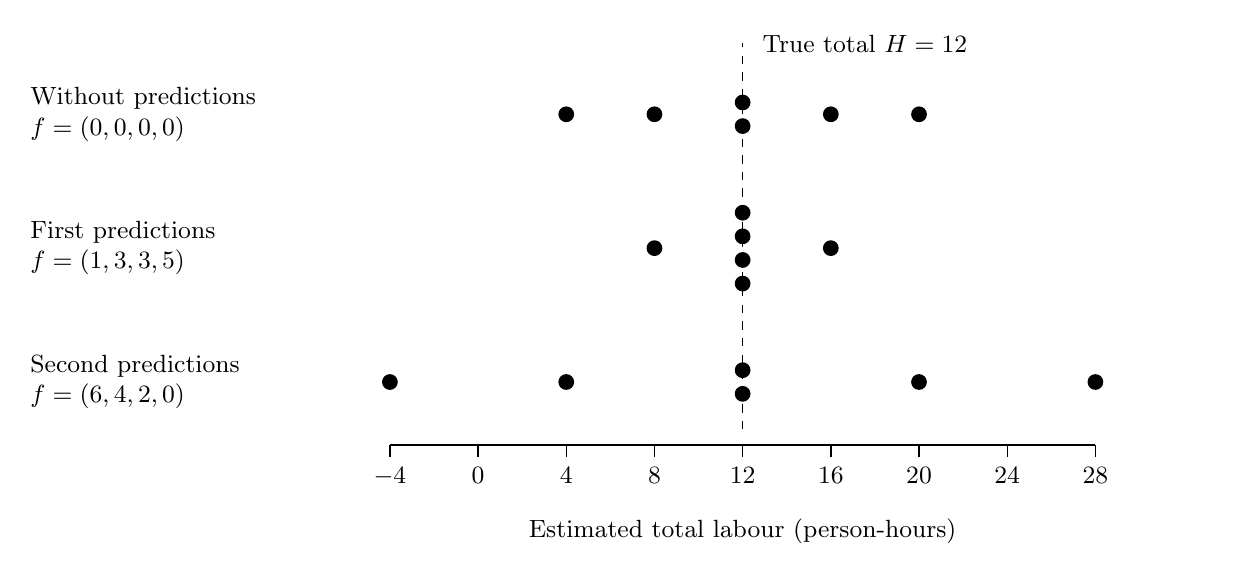
\begin{tikzpicture}[x=1mm,y=1mm,font=\fontsize{9}{11}\selectfont,
  every node/.style={inner sep=1pt,outer sep=0pt}]
  \path[use as bounding box] (0,-9) rectangle (152.4,58);
  \draw[dashed,line width=0.6pt] (90.8,7) -- (90.8,56);
  \node[anchor=west] at (93,56) {True total $H=12$};
  \node[anchor=west,align=left] at (0,47) {Without predictions\\$f=(0,0,0,0)$};
  \node[anchor=west,align=left] at (0,30) {First predictions\\$f=(1,3,3,5)$};
  \node[anchor=west,align=left] at (0,13) {Second predictions\\$f=(6,4,2,0)$};
  \foreach \estimate/\offset in {4/0,8/0,12/-1.5,12/1.5,16/0,20/0} {
    \fill ({46+2.8*(\estimate+4)},{47+\offset}) circle (1mm);
  }
  \foreach \estimate/\offset in {8/0,12/-4.5,12/-1.5,12/1.5,12/4.5,16/0} {
    \fill ({46+2.8*(\estimate+4)},{30+\offset}) circle (1mm);
  }
  \foreach \estimate/\offset in {-4/0,4/0,12/-1.5,12/1.5,20/0,28/0} {
    \fill ({46+2.8*(\estimate+4)},{13+\offset}) circle (1mm);
  }
  \draw[line width=0.5pt] (46,5) -- (135.6,5);
  \foreach \estimate in {-4,0,4,8,12,16,20,24,28} {
    \draw[line width=0.5pt] ({46+2.8*(\estimate+4)},5)
      -- ({46+2.8*(\estimate+4)},3.5);
    \node[anchor=north] at ({46+2.8*(\estimate+4)},2.5) {$\estimate$};
  }
  \node at (90.8,-6) {Estimated total labour (person-hours)};
\end{tikzpicture}
\caption{\textbf{The estimates have the same average but vary differently across samples.}
For the hypothetical labour values $y=(0,2,4,6)$, each dot shows the estimated total from one of the six equally likely samples of two person-intervals, meaning time intervals for individual people. Dots at the same value are stacked so every sample is visible. Each row averages to the true total of twelve person-hours. Predictions $f=(1,3,3,5)$ reduce variation across samples relative to estimation without predictions. Predictions $f=(6,4,2,0)$ increase that variation and can produce a negative estimate. Each row shows all six samples and the estimate calculated from each.}
\label{fig:sampling-spread}
\end{figure}
